\documentclass[openany]{article}

%Standard Stefanos Packages
\usepackage[utf8]{inputenc}
\usepackage{dirtytalk}
\usepackage{amsmath}
\usepackage{mathtools}  
\mathtoolsset{showonlyrefs} 
\usepackage{graphicx}
\usepackage{mdframed}
\usepackage{lipsum}
\usepackage{cancel}
\usepackage{systeme}
\usepackage{pgfplots}
\usepackage{textcomp}
\usepackage{geometry}
\usetikzlibrary{arrows}
\geometry{a4paper}
\graphicspath{ {./res/} }
\usepackage{float}
\restylefloat{table}
\newcommand{\comment}[1]{%
	\text{\phantom{(#1)}} \tag{#1}
}
\title{\line(1,0){450}\\ ST3MVA Multivariate Data Analysis (2020/21) \\ \large Coursework 2  \\\line(1,0){450} \\ }
\usepackage{pgfplots}
\author{Stefanos Stefanou}
\newmdtheoremenv{note}{Note}
\pgfplotsset{compat=1.17}

%Extra Packages
\usepackage{tikz}
\usetikzlibrary{automata,positioning}
\geometry{margin=0.5in}
\usepackage{listings}
\usepackage{xcolor}

\definecolor{dkgreen}{rgb}{0,0.6,0}
\definecolor{gray}{rgb}{0.5,0.5,0.5}
\definecolor{mauve}{rgb}{0.58,0,0.82}

\lstdefinestyle{myScalastyle}{
	frame=tb,
	language=scala,
	aboveskip=3mm,
	belowskip=3mm,
	showstringspaces=false,
	columns=flexible,
	basicstyle={\small\ttfamily},
	numbers=none,
	numberstyle=\tiny\color{gray},
	keywordstyle=\color{blue},
	commentstyle=\color{dkgreen},
	stringstyle=\color{mauve},
	frame=single,
	breaklines=true,
	breakatwhitespace=true,
	tabsize=3,
}


\begin{document}
	\section{Exploration}
		A first step in every data analysis task, is the exploration part. Lets draw a scatterplot matrix
		\begin{figure}[H]
			\iftrue
			\begin{lstlisting}[style=myScalastyle]
my_cols <- c("red", "green", "blue","yellow", "black", "purple","pink") 
fish<-read.csv("FishNum.csv")
data <- fish[ , c(3:7,9)]
category<-unclass(fish[,2])
sex <- fish[,8]
pairs(main="ID : 27020363",data, pch = c(1,4,13)[sex],  cex = 1,
col = my_cols[unclass(category)],
lower.panel=NULL)
			\end{lstlisting}
			\fi
		\end{figure}
		\begin{figure}[H]
			\iftrue
			\caption{Scatterplot Produced}
			\centering
			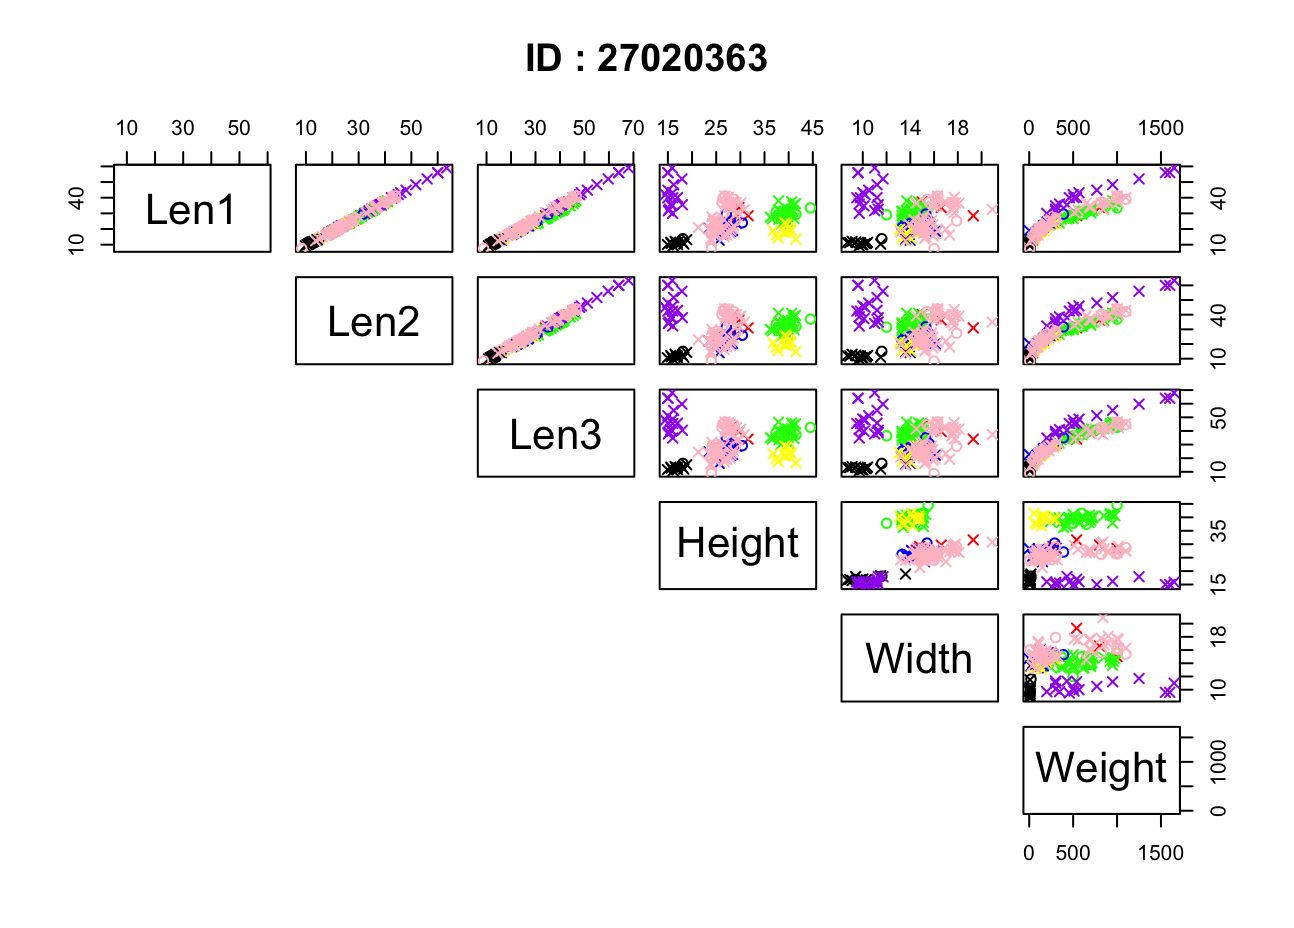
\includegraphics[scale=0.4]{res/matrixscatter}
			\fi
		\end{figure}
		Multiple things are happening here. Colour represents species, and shape point represents the sex of a given observation. Due to the number of given
		combinations(2 states of sex (male/female/NA) times 7 categories = 14) , Instead of a legend, a detailed table is given below.
		\begin{center}
			
			\begin{tabular}{ c c }
				Red & Whitewish  \\ 
				Green & Bream \\ 
				Blue & Roach \\ 
				Yellow & Parkki\\ 
				Black & Smelt\\ 
				Purple & Pike\\ 
				Pink & Perch\\ 
			\end{tabular}
			\begin{tabular}{ c c }
				
\includegraphics[scale=0.4]{res/1} & male  \\ 
				
\includegraphics[scale=0.4]{res/4} & female  \\ 
				
\includegraphics[scale=0.4]{res/13} & N/A  \\ 
			\end{tabular}
		\end{center}
		\subsection{Intepretation of Scatterplot matrix}
			The scatterplot matrix is, in fact, messy. There is not a single species that distinguishes itself from the others. Fortunately, there is plenty 
			of room for valuable information extraction by separating groups of species.
			\begin{itemize}
				\item We may use LenN vs LenM (Len1,Len2,Len3) To separate female Pike fish, as we can see they are the only fish passing a specific thresold
				\item We may use Height to separate Group(Pike , Smelt) from the rest of the species. Adding a LenM variable (Len1,Len2,Len3) (using the y axis) we can further separate Pike, Smelt from each other.Unfortunately this is not the case for Group(Bream,Parkki) as there is a subtle overlap.
				\item We may use Weight vs Width and Height vs Width to separate Group(Smelt,Pike) and Group(Bream,Parkki) from the rest of the species.
			\end{itemize} 
	\section{Classification Rules}
		As we already know the groups, the best approach is to create and intepret Canonical Variates, as seen below
		\begin{figure}[H]
			\iftrue
			\begin{lstlisting}[style=myScalastyle]
> lmdata<-lm(cbind(Len1, Len2, Len3, Height, Width,Weight) ~ Species)
> lmdata<-candisc(lmdata, term='Species')
> cv<-lmdata$coeffs.std
> cv
              Can1        Can2         Can3        Can4         Can5         Can6
Len1    -1.8998871   4.7292421 -13.47872399  -3.0661783 -20.10853177 -19.75182360
Len2   -15.1471855  10.0001971  19.98611329 -11.0463562  22.23620080  20.80689533
Len3    17.1207575 -16.1854062  -4.04204695  13.4266478  -3.42658135  -0.83968837
Height   0.9932291   0.5230676   0.07445439  -0.5298317  -0.04932795  -0.04162895
Width   -0.4803954   0.4001957   0.39911882   0.9424763  -0.24174065  -0.15612550
Weight  -0.2726642   0.9055450  -2.27768564   0.4630591   1.85263470  -0.94857277
			\end{lstlisting}
			\fi
		\end{figure}
		Lets jump in straight into a scores plot!
		\begin{figure}[H]
			\iftrue
			\begin{lstlisting}[style=myScalastyle]
>plot(scores[,2],scores[,3],main="ID : 27020363",xlab='canonical variate 1',ylab='canonical variate 2',col=my_cols[fishNum$Species],pch=c(1,4,13)[sex])
			\end{lstlisting}
			\fi
		\end{figure}
		\subsection{CV1 vs CV2}
			\begin{figure}[H]
				\iftrue
				\caption{CV Scores plot}
				\centering
				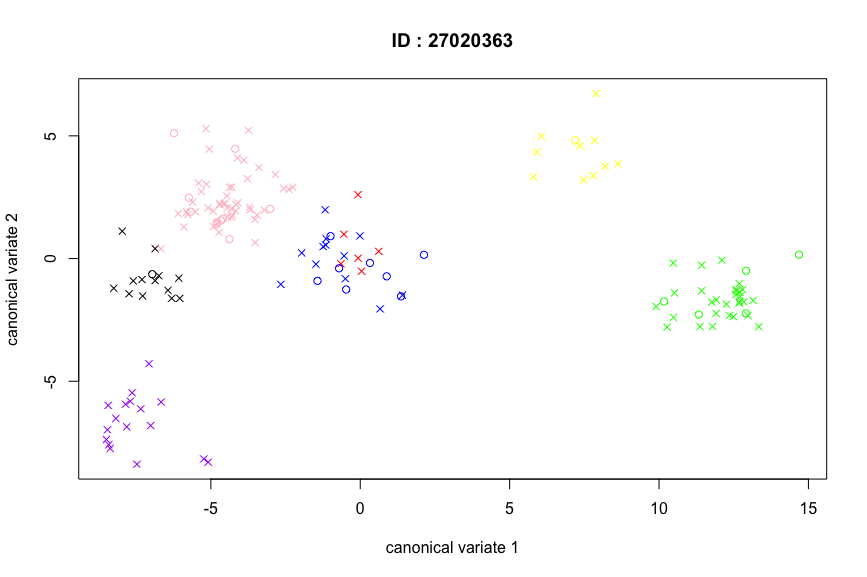
\includegraphics[scale=0.2]{res/cv}
				\fi
			\end{figure}
			\subsubsection{CV1}
				For the first canonical variate, we can see the Len2 and Len3 are driving with their extreme values, Len1 and Height are considered somewhat influencial
				with the rest of the variables to be deemed not influencial(0.3 rule of thumb is not a sufficient rule here, as Len2 and Len3 have extreme values).
				Using the CV1, We can easily separate our observations using CV1 into the following categories.
				\begin{center}
					
					\begin{tabular}{ c c c c }
						\title{Rules extracted from CV1}
						&(Bream or Parkki) &$\rightarrow$& Compartively large Len3 scores  \\ 
						&(Roach or Smelt or Pike or Perch) &$\rightarrow$& Compartively small scores of Len2 \\ 
					\end{tabular}
				\end{center}
			\subsubsection{CV2}
				We can further classify Pike by introducing PC2 on y axis,
				\begin{center}

					\begin{tabular}{ c c c }
						\title{Rules extracted from CV2}
						Pike & $\rightarrow$ &Compartively small Len3 and Len2 scores  \\ 
					\end{tabular}
				\end{center}
				Given our previous observation, Perch seems to always have relatively small scores for both Len2 and Len3
		\subsection{CV2 vs CV3}
			\begin{figure}[H]
			\iftrue
				\begin{lstlisting}[style=myScalastyle]
				>plot(scores[,3],scores[,4],main="ID : 27020363",xlab='canonical variate 2',ylab='canonical variate 3',col=my_cols[fishNum$Species],pch=c(1,4,13)[sex])
				\end{lstlisting}
				\fi
			\end{figure}	
			\begin{figure}[H]
				\iftrue
				\caption{CV Scores plot}
				\centering
				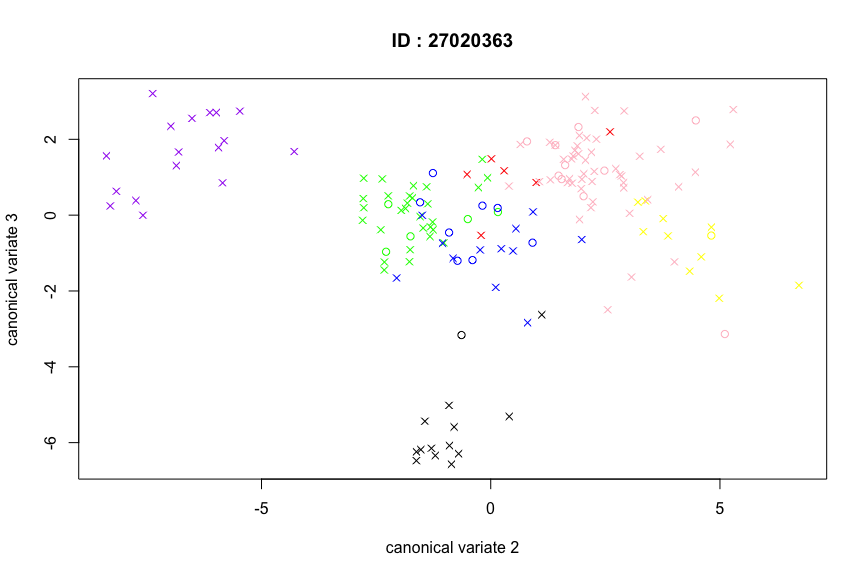
\includegraphics[scale=0.2]{res/cv23}
				\fi
			\end{figure}
			\subsubsection{CV3}
				Using CV3, we can observe that Smelt fishes have relatively small scores on Len1 variable. Unfortunaly due to the mixing other observations, we 
				cant further separate any other groups when adding CV3.
				\begin{center}
					\begin{tabular}{ c c c }
						\title{Rules extracted from CV2}
						Smelt & $\rightarrow$ &Compartively small Len1 scores  \\ 
					\end{tabular}
				\end{center}
			Unfortunately, There is no other interesting separations on other CV's. Lets sum up our rules
		\subsection{Summing and Merging our Rules}
			\begin{tabular}{ c c c c }
				&(Bream or Parkki) &$\rightarrow$& Compartively large Len3 scores  \\ 
				&(Roach or Perch) &$\rightarrow$& Compartively small scores of Len2 \\ 
				&Pike & $\rightarrow$ &Compartively small Len3 and Len2 scores  \\
				&Smelt & $\rightarrow$ &Compartively small Len1 and Len2 scores  \\  
			\end{tabular}
	\section{Classification}
		In order to classify a new observation, we will perform Fishers linear discriminant analysis. On the first step, we need a matrix to obtain the medians 
		for each group and variable. 
		\begin{figure}[H]
			\iftrue
			\begin{lstlisting}[style=myScalastyle]
> aggregate(data_and_categories , list(Species), FUN=mean) [,c(1,3:8)]
    Group.1     Len1     Len2     Len3   Height    Width    Weight
1     Bream 30.32941 33.14118 38.38529 39.59118 14.14706 626.00000
2    Parkki 18.72727 20.34545 22.79091 39.30909 14.08182 154.81818
3     Perch 26.00526 28.17544 29.87018 26.26667 15.84737 393.07719
4      Pike 42.47647 45.48235 48.71765 15.84118 10.43529 718.70588
5     Roach 20.64500 22.27500 24.97000 26.73500 14.60500 152.05000
6     Smelt 11.25714 11.92143 13.03571 16.88571 10.22143  11.17857
7 Whitewish 28.80000 31.31667 34.31667 29.20000 15.90000 531.00000
			\end{lstlisting}
			\fi
		\end{figure}
		We also need the raw coefficients
		\begin{figure}[H]
			\iftrue
			\begin{lstlisting}[style=myScalastyle]
> lmdata$coeffs.raw
                Can1         Can2         Can3        Can4         Can5         Can6
Len1   -0.2901615702  0.722276748 -2.058547385 -0.46828419 -3.071089335 -3.016610835
Len2   -2.1811348411  1.439988859  2.877921315 -1.59063163  3.201925022  2.996110684
Len3    2.3318809609 -2.204484278 -0.550534773  1.82873593 -0.466707144 -0.114367213
Height  0.6211299020  0.327107741  0.046561110 -0.33133777 -0.030847934 -0.026033254
Width  -0.4362075050  0.363384704  0.362406900  0.85578503 -0.219504757 -0.141764701
Weight -0.0009313501  0.003093106 -0.007779982  0.00158169  0.006328119 -0.003240078			
			\end{lstlisting}
			\fi
		\end{figure}
		Let the following observation
		\begin{center}
			
			\begin{tabular}{ c c c c c c }
				Len1  &   Len2  &   Len3 &  Height  &  Width  &  Weight \\
				31.7  &   34    &   37.8 &  15.1    & 11      &  300
				
			\end{tabular}
		\end{center}
		We can produce at most 5 discriminant functions. Our first discriminant function for CV1 will have the form
		\begin{align}
			y=-0.29\cdot\text{Len1}-2.181\cdot\text{Len2}+2.331\cdot\text{Len3}+0.621\cdot\text{Height}-0.436\cdot\text{Width}-0.0009\cdot\text{Weight}\\
			y_{\text{Bream}}=-0.29\cdot 30.32-2.181\cdot 33.14+2.331\cdot 38.38+0.621\cdot 39.59-0.436\cdot 14.147-0.0009\cdot 626 = 28.42\\
			y_{\text{Parkki}}=-0.29\cdot 18.72-2.181\cdot 20.34+2.331\cdot 22.79+0.621\cdot39.30-0.436\cdot 14.08-0.0009\cdot 154.81 = 41.24\\
			y_{\text{Perch}}=-0.29\cdot 26.00-2.181\cdot 28.17+2.331\cdot 29.87+0.621\cdot 26.26-0.436\cdot 15.84-0.0009\cdot 393.077 = 8.38\\
			y_{\text{Pike}}=-0.29\cdot 42.47-2.181\cdot 45.48+2.331\cdot 48.71+0.621\cdot 15.84-0.436\cdot 10.43-0.0009\cdot 718.705 = 6.67 \\
			y_{\text{Roach}}=-0.29\cdot 20.64-2.181\cdot 22.27+2.331\cdot 24.97 +0.621\cdot 26.73 -0.436\cdot 14.60 -0.0009\cdot 152.050 =13.74\\
			y_{\text{Smelt}}=-0.29\cdot 11.25 -2.181\cdot 11.92 +2.331\cdot 13.03 +0.621\cdot 16.88 -0.436\cdot 10.22 -0.0009\cdot 11.17 = 7.12\\
			y_{\text{Whitewish}}=-0.29\cdot 28.80-2.181\cdot 31.31 +2.331\cdot 34.31 +0.621\cdot 29.20 -0.436\cdot 15.90 -0.0009\cdot 531.00 = 14.06\\
		\end{align}
		We can already predict our observation without the additional steps, as follows.
		\begin{align}
			y^*=-0.29\cdot 31.7 -2.181\cdot 34 +2.331\cdot 37.8+0.621\cdot 15.1 -0.436\cdot 11-0.0009\cdot 300\\
			y^*=9.0759
		\end{align}
		Our new observation is between Perch(8.38) and Roach(13.74). Is significantly closer to Perch, so we classify it as Perch.
			
	
\end{document}